\begin{rep}% AR
La vraisemblance s'écrit  
\begin{eqnarray*}
f({\bf x_n}|\theta) & \propto & \underbrace{\exp\left(-\frac{1}{2}\sum\limits_{k=1}^{n-1} (x_k-\theta)^2\right)}_{\text{\tiny terme régulier}} \ \ \ \left(\underbrace{1-\Phi(y-\theta)}_{\text{\tiny \begin{tabular}{l} terme dû à la censure \\ $\ \ = \ P(X>y)$ \end{tabular}}}\right).  
\end{eqnarray*}
L'{\it a posteriori} sur $\theta$ s'écrit alors
\begin{eqnarray*}
\pi(\theta|{\bf x_n}) & \propto & \tilde{\pi}(\theta|{\bf x_n}) \ = \ \exp\left\{-\frac{n}{2}\left[\theta - \frac{1}{n}\left(\mu + \sum\limits_{k=1}^{n-1} x_k\right)\right]^2\right\}\left\{1-\Phi(y-\theta)\right\}. 
\end{eqnarray*}
On remarque que si $y=x_n$, on aurait un modèle conjugué et $\pi(\theta|{\bf x_n})$ serait une loi normale. Il semble donc pertinent de proposer, comme choix de loi instrumentale,
$$
\rho(\theta) \equiv {\cal{N}}\left(\frac{1}{n}\left(\mu + \sum\limits_{k=1}^{n-1} x_k\right),1/n\right).
$$
Puisque $1-\Phi(y-\theta)\leq 1$, on a
\begin{eqnarray*}
\tilde{\pi}(\theta|{\bf x_n}) & \leq & \underbrace{\sqrt{\frac{2\pi}{n}}}_{K} \cdot\{1-\Phi(y-\theta)\}\cdot\rho(\theta).
\end{eqnarray*}
On peut donc mettre en oeuvre l'algorithme comme suit : on accepte $\theta_i$ si $U_i\leq 1-\Phi(y-\theta_i)$. Le nombre moyen d'appels nécessaires à $\rho(\theta)$ varie proportionnellement à $1/\sqrt{n}$, donc
plus l'échantillon de données grandit, plus l'algorithme est efficace.
Si cependant, on fait le choix $\rho(\theta)=\pi(\theta)$, alors
\begin{eqnarray*}
K & = & \sqrt{2\pi}\exp\left(\frac{1}{2}\left[\frac{1}{n-1}\sum\limits_{k=1}^n x_k - \mu\right](1-\sqrt{n})\right) 
\end{eqnarray*}
Voir la figure \ref{ARillus} pour une illustration de la mise en oeuvre de cet algorithme.
\end{rep}

\begin{figure}[hbtp]
\begin{center}
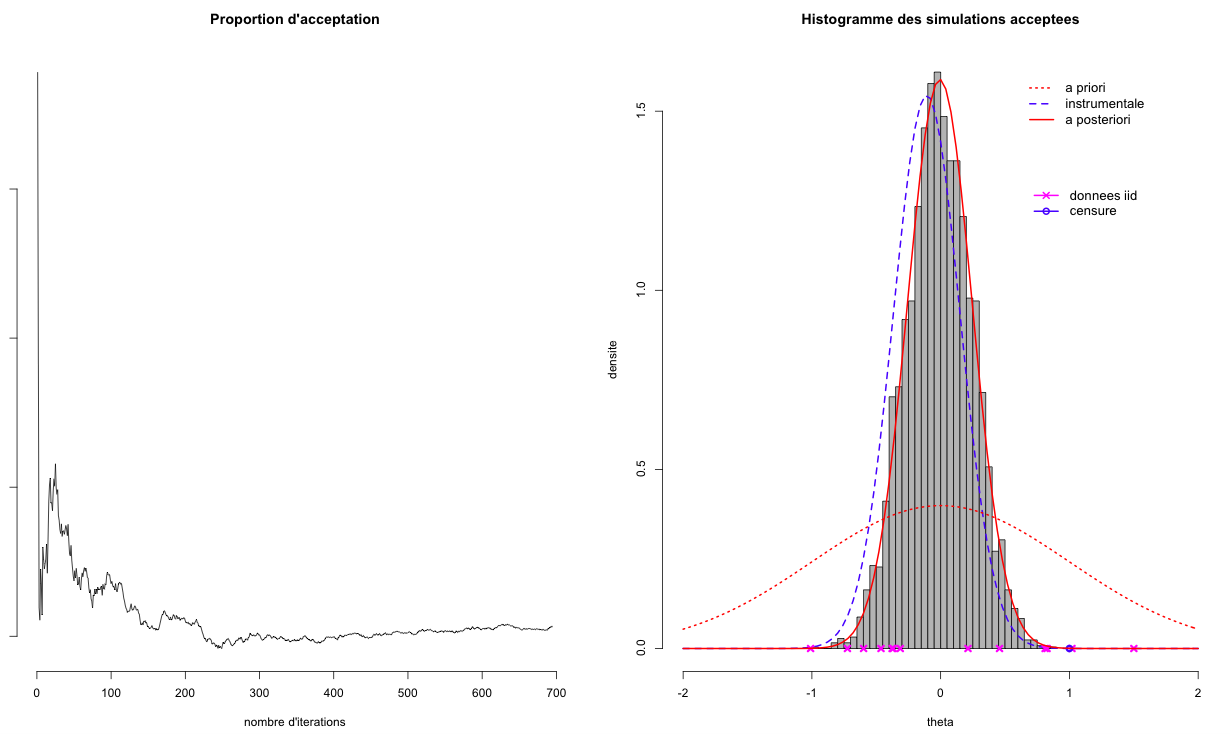
\includegraphics[scale=0.3]{figures/calcul/AR1.png} \\
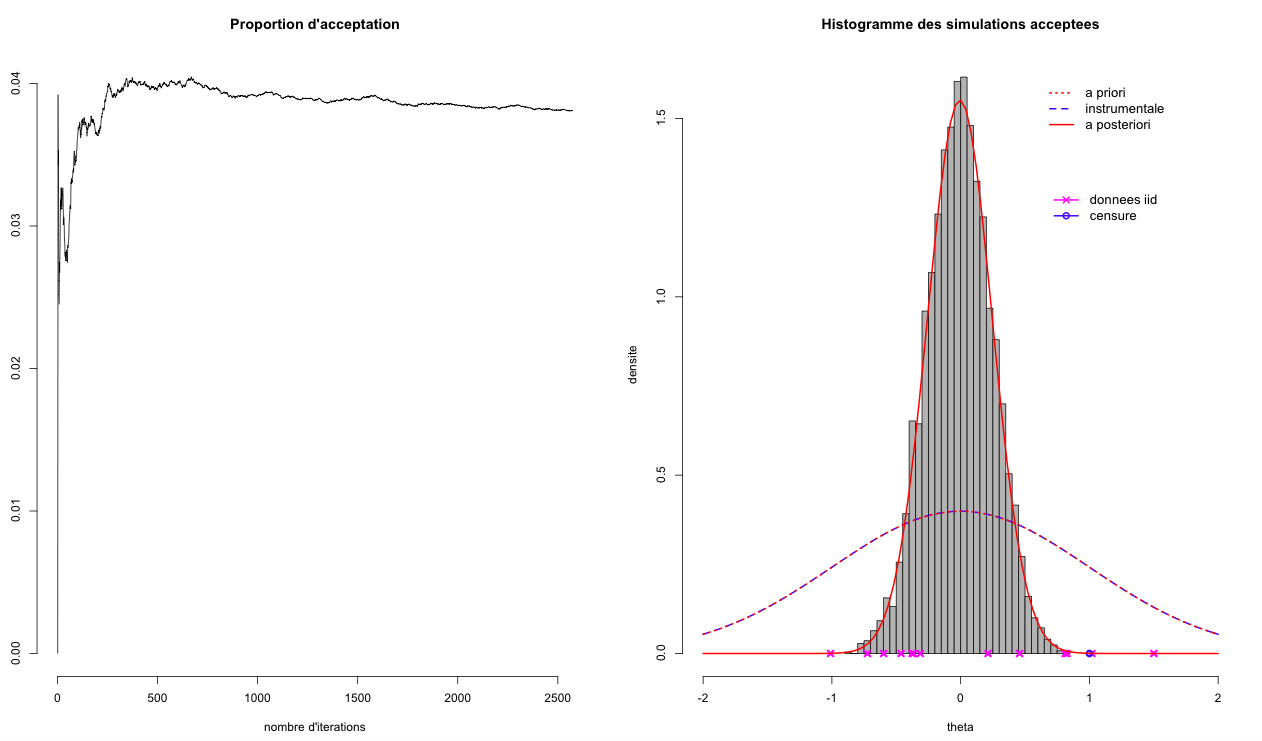
\includegraphics[scale=0.3]{figures/calcul/AR2.png}
\caption{
Essai de simulation par AR en utilisant (en haut) une loi instrumentale ``proche" du vrai posterior ; (en bas) le prior comme loi instrumentale.}
\label{ARillus}
\end{center}
\end{figure}
